\documentclass{article}
\usepackage[utf8]{inputenc}
% \usepackage[russian]{babel}
\usepackage[a4paper, top=0.7in, left=0.5in, right=0.5in, bottom=0.6in, twocolumn]{geometry}
\usepackage{lastpage}
\usepackage{fancyhdr}
\usepackage{tikz}
\usepackage{pgfplots}
\usepackage{amssymb}
\usepackage{minted}
\usepackage{pdfpages}
\usepackage{booktabs}
\usepackage{hyperref}
\usepackage{amsmath}

\usetikzlibrary{shapes}

\setcounter{secnumdepth}{5}
\setcounter{tocdepth}{5}
\pgfkeys{/pgf/number format/.cd,1000 sep={\,}}

\pagestyle{fancy}
\fancyhf{}
\lhead{ITMO University 1: Standard deviation (Budin, Kirillov, Sayutin)}
\rhead{Page \thepage\ of \pageref{LastPage}}
\lfoot{Generated \today}

\renewcommand{\footrulewidth}{0.4pt}
\setlength{\columnseprule}{0.4pt}

\begin{document}
% \onecolumn
\tableofcontents

% \twocolumn
\newpage

% Content

\onecolumn
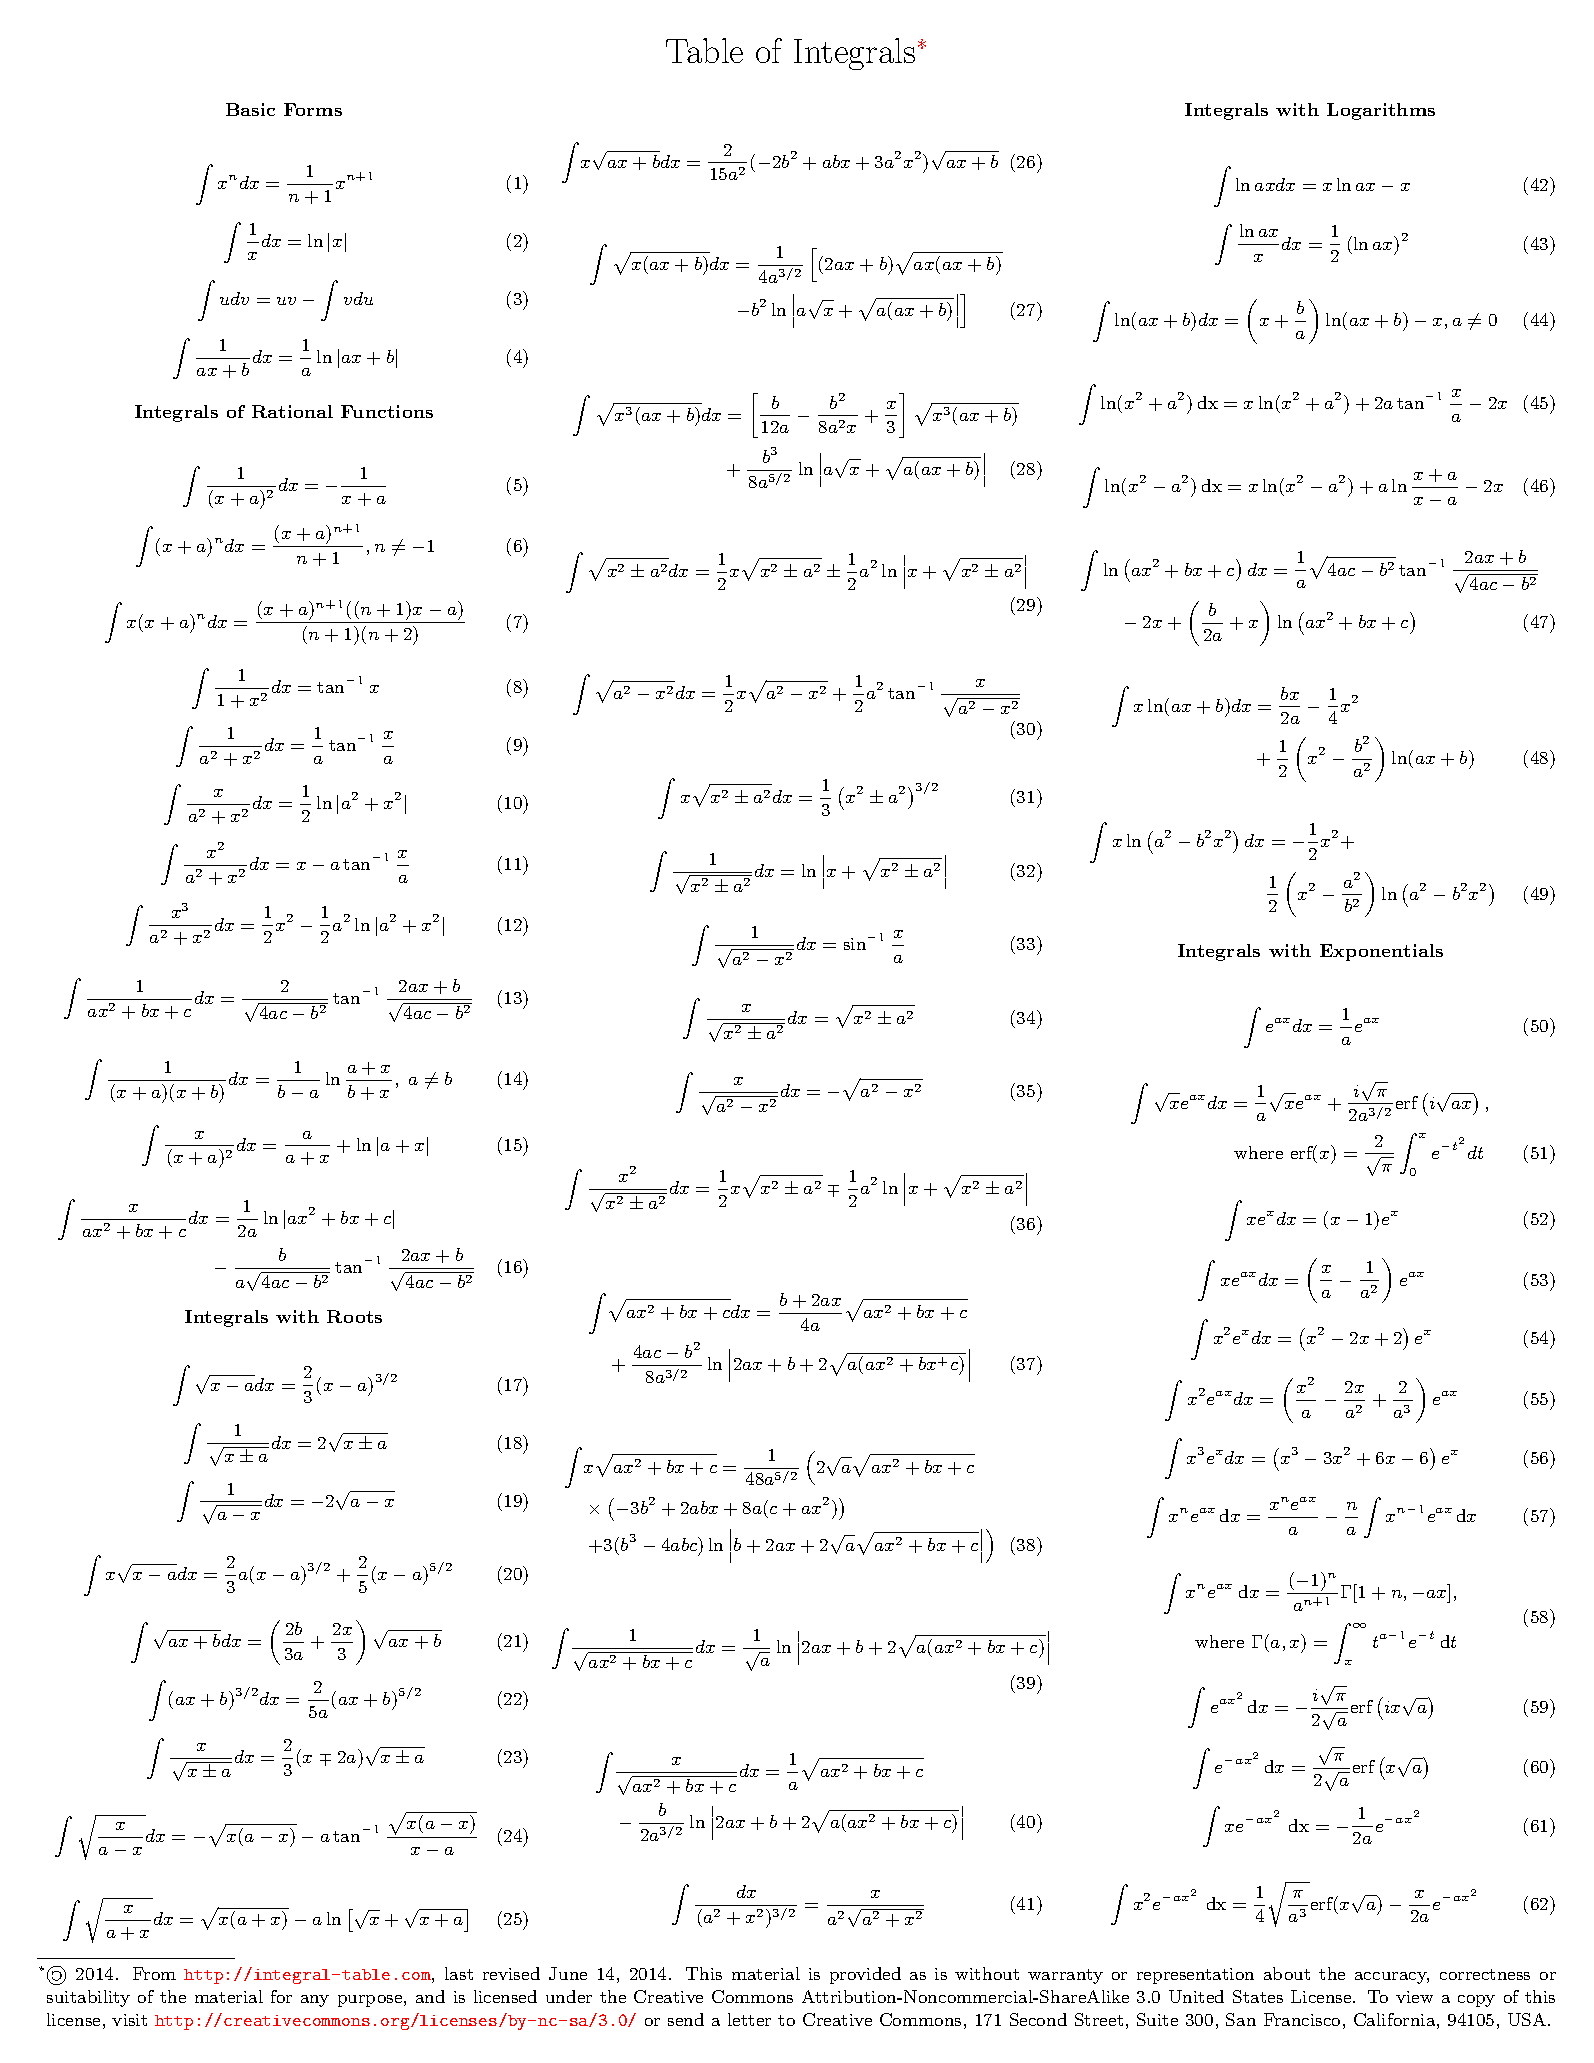
\includepdf[pages={1, 2}, pagecommand={\pagestyle{fancy}}]{integral-table}

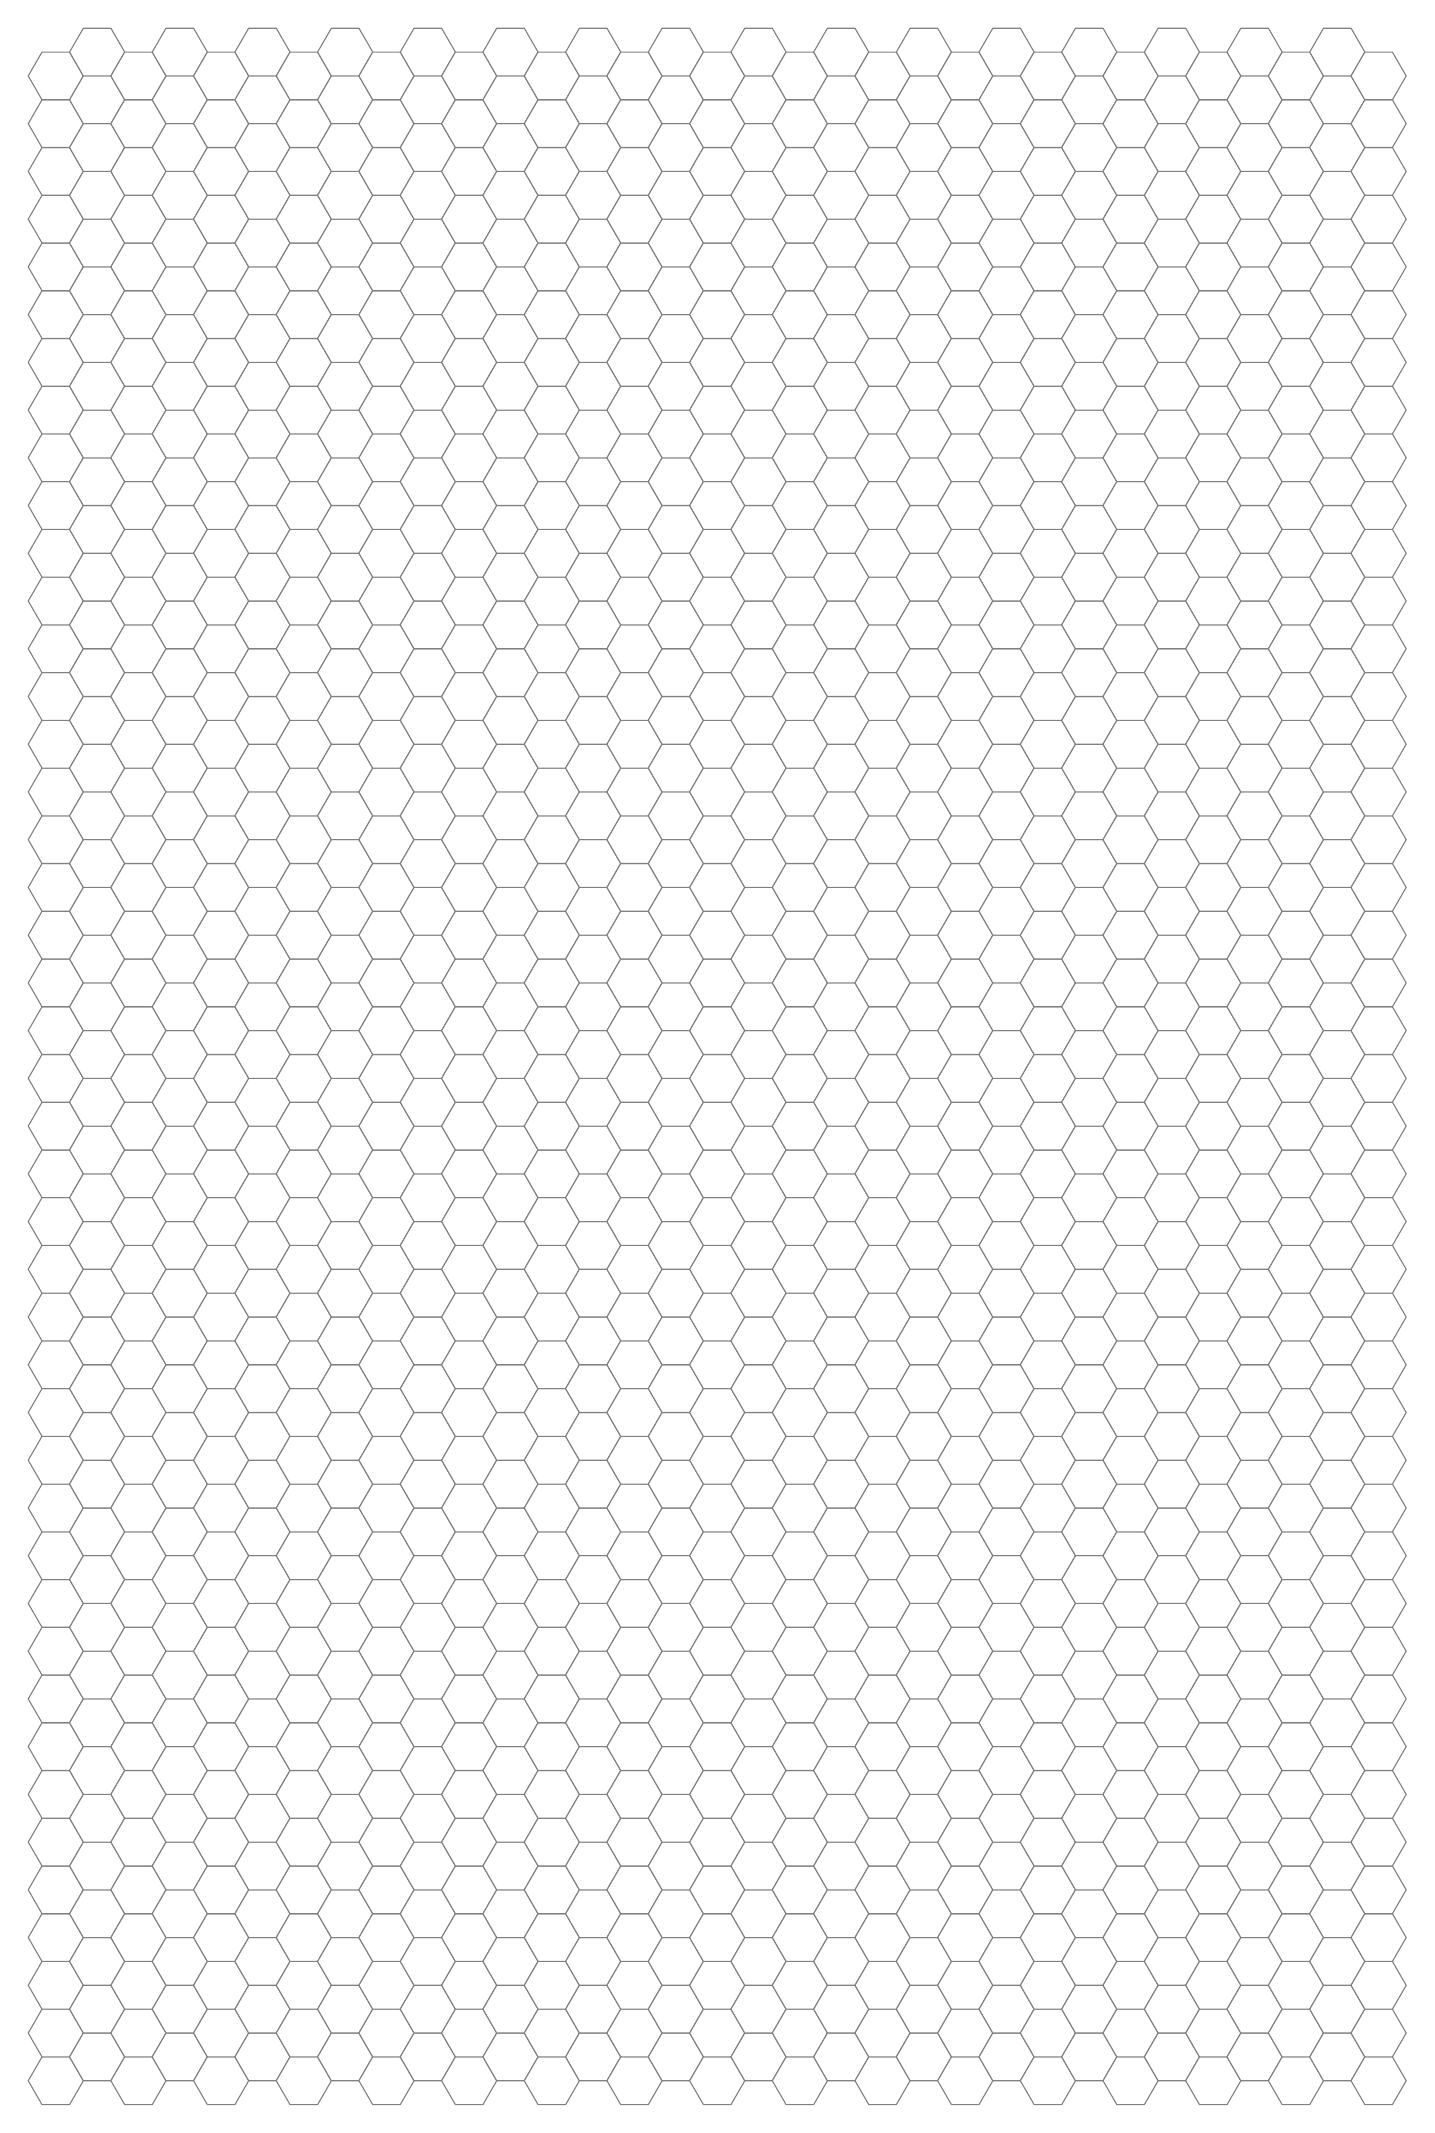
\begin{tikzpicture} [hexa/.style= {shape=regular polygon,
                                   regular polygon sides=6,
                                   minimum size=0.7cm, draw=gray,
                                   inner sep=0, anchor=south,
                                   fill=white}]

\foreach \j in {0,...,32}{% 
    \ifodd\j 
         \foreach \i in {0,...,42}{\node[hexa] (h\j;\i) at ({(\j/2+\j/4) * 0.7},{(\i+1/2)*sin(60) * 0.7}) {};}        
    \else
         \foreach \i in {0,...,42}{\node[hexa] (h\j;\i) at ({(\j/2+\j/4) * 0.7},{\i*sin(60) * 0.7}) {};}
    \fi}
\end{tikzpicture}

\end{document}